\documentclass[12pt,letterpaper,titlepage]{article}
\usepackage{solarized-light}

\usepackage{fontspec}
\defaultfontfeatures{Mapping=tex-text}
\usepackage{xunicode}
\usepackage{xltxtra}
\usepackage{amsmath}
\usepackage{pdfpages}
\usepackage{amsfonts}
\usepackage{amssymb}
\setcounter{secnumdepth}{0}
\usepackage{nameref}
\usepackage{enumitem}
\usepackage{pgfplots}

\setmainfont{Times New Roman}
\showboxdepth=\maxdimen
\showboxbreadth=\maxdimen

\usepackage[tocflat]{tocstyle}
\usetocstyle{allwithdot}
\usepackage[bottom]{footmisc}
\pgfplotsset{compat=1.15}
\usepackage{karnaugh-map}
\usepackage{paracol}
\usepackage{wrapfig}
\globalcounter{table}
\globalcounter{figure}
\usepackage{graphicx}
\usepackage[left=1in,right=1in,top=1in,bottom=1in]{geometry}
\graphicspath{{img/}}
\lstset{language=c}

\author{Jacob Abel}
\title{	Homework 4
	\\\large ECE2534 CRN:12927
}

\setlength{\parskip}{0.5em}

\begin{document}
\maketitle

\begin{raggedright}

\paragraph{Problem 1: } 
Consider a UART with the following setup: 
\begin{itemize}[noitemsep]
\item 8 data bits
\item EVEN parity
\item 2 stop bits
\item LSB first.
\end{itemize}

\begin{enumerate}[label=\alph*)]
\item If the receiver gets the following frame: 111100111011001111, has there been any data corruption in this communication? Explain and show your work to a reasonable extent.

Start Bit: 0, Data: 01110110, Parity Bit: 0, Stop Bits: 11, Hamming Weight: 5 (Odd)

The start and stop bits are correct however the data has the incorrect parity. There was likely data corruption.

\item If the baudrate is 9600 baud/sec, approximately how long does it take to transfer one character using this UART?

$\frac{1}{9600}s\approx 104\mu s$

\item If one end wishes to send 'G' to another, what will be the full data frame including start, data, parity and stop bits?

Start Bit: 0, Data: 0x47 : 1110001, Hamming Weight: 4 (Even), Parity Bit: 0, Stop Bits: 11

01110001011

\end{enumerate}

\clearpage
\paragraph{Problem 2: } 
Consider a UART with the following setup: 
\begin{itemize}[noitemsep]
\item 8 data bits
\item Odd parity
\item 1 stop bit
\item LSB first
\item BRCLK (Baudrate Source Clock) is 2.88 MHz
\item Baudrate is 460800 bit/sec
\end{itemize}

\begin{enumerate}[label=\alph*)]
\item For the MSP432 UART calculate the values of BCRx and BCRSx. (Based on the footnote below the Table 24-4 of MCU User Guide, if the fraction part of the division factor falls between two values in the table, we need to pick the lower one. In the Lab 2 starter code, we made a small mistake when by choosing 0xAA instead of 0x55. For this problem, please follow the proper method for selecting BCRSx)

\begin{align*}
   N &= \frac{2.88MHz}{460800bit/sec} = 6.25
\\ OS16 &= 0
\\ UCBRx &= 6
\\ UCBRSx &= 0x22
\end{align*}

\pagebreak
\item If we mark the middle of the start bit as beginning of time (0 $\mu$s), then,
\begin{enumerate}[label=\roman*), noitemsep]
\item When is the ideal ​moment for sampling each of the following bits?
\item What is the counter value that UART should load at each sampling moment (for waiting until next sampling moment)?
\item What is the total ​"clock ticks" UART has waited up to each sampling moment?
\item What is the actual ​sampling moment for each bit?
\item What is the error (difference) between the ideal and actual sampling times?
\end{enumerate}
Use the table below to enter your answers. For sampling times and error, enter the numbers in microseconds with two decimal points accuracy. The first three rows are completed to guide you.


\begin{tabular}{|c|c|c|c|c|c|}
\hline 
          & Ideal time & Counter value & Total ticks & Actual time &  \\ 
Bit Index & to sample  & to be loaded  & waited      & to sample   & Error \\\hline 
 0 &  0.00 & 6 &  0 &  0.00 &  0.00 \\\hline
 1 &  2.17 & 6 &  6 &  2.08 & -0.09 \\\hline
 2 &  4.34 & 7 & 12 &  4.17 & -0.17 \\\hline
 3 &  6.51 & 6 & 19 &  6.60 & +0.09 \\\hline
 4 &  8.68 & 6 & 25 &  8.68 &  0.00 \\\hline
 5 & 10.85 & 6 & 31 & 10.77 & -0.08 \\\hline
 6 & 13.02 & 7 & 37 & 12.85 & -0.17 \\\hline
 7 & 15.19 & 6 & 50 & 15.28 & +0.09 \\\hline
 8 & 17.36 & 6 & 56 & 17.36 &  0.00 \\\hline
 9 & 19.53 & 6 & 62 & 19.44 & -0.09 \\\hline
10 & 21.70 & 7 & 68 & 21.53 & -0.17 \\\hline
\end{tabular} 

\item In a few sentences explain how you use your response to part a to answer part b.ii?

UCBRx is the default counter value and UCBRSx is the modulation bitmap. (i.e. Convert 0x22 to binary, mask all but the i\%8 bit and if the value is nonzero, increment the counter value for the next iteration)
\pagebreak
\item Graph the error values with respect to bits. Do you see a pattern? Explain in a few words.
	\begin{tikzpicture}
	\begin{axis}[
		title=UART Error,
		axis lines = left,
		width=0.8\textwidth,
		ylabel near ticks,
		xlabel = $Bit\;Index$, 
		ylabel = $Error(\mu s)$,
		tick label style={/pgf/number format/fixed},
		legend style={empty legend},
		legend pos = north west]]
\addplot[
    color=blue,
    mark=square,
    ]
    coordinates {
    (0,0)(1,-0.09)(2,-0.17)(3,0.09)(4,0)(5,-0.08)(6,-0.17)(7,0.09)(8,0)(9,-0.09)(10,-0.17)
    };
	\end{axis}
	\end{tikzpicture}
	
	
The error is very periodic and always corrects every 4 bits.
\end{enumerate}

\clearpage
\paragraph{Problem 3: }
Consider a 32-bit Timer that is ticking with a 10MHz clock. Answer the following questions:

\begin{enumerate}[label=\alph*)]
\item In the one-shot mode, to measure 500 ms, what is the value that needs to be loaded to the counter of this timer?

$10MHz \times 500ms = 5000000$

\item In the one-shot mode, if we load 1000 in the counter, how long does it take before the timer expires?

$\frac{1000}{10MHz} = 100\mu s$

\item What is the longest amount of time that can be measured in the one-shot mode using this timer?

$\frac{2^{32}-1}{10MHz} = 429.5s$

\item In the periodic mode with N = 10,000

\begin{enumerate}[label=\roman*)]
\item If we read the counter, and it is 3000, if we wait for 7000 clock ticks, and read the counter again, what is the expected counter value (approximately)?

It should be at 6000 as it burnt the 3000 ticks, reset back to 10000, and burnt the remaining 4000 ticks.

\item If we read the counter, and it is 4000, what is the counter value after 0.5 ms?

$10MHz \times 0.5ms = 5000\implies 4000 - 5000 = -1000 \implies 10000-1000=9000$ The counter will be at 9000.

\item If we read the counter value, and it is 2000 , and then we read it again, and it is 4000, and we know for sure the clock has rolled over only once during this time, how long has passed?

$2000 + (10000-4000) = 8000\implies \frac{8000}{10MHz} = 800\mu s$

\end{enumerate}
\end{enumerate}

\clearpage
\paragraph{Problem 4: }
The below snippet of code starts TIMER32\_0\_BASE in free running mode with the max possible period. You need to write a function that uses this function to measure a given amount of time in microseconds. The details of the function are provided below.

\begin{lstlisting}
// 16-bit timer ticking at 3,000,000 Hz
// Free running (periodic mode) with N equal to 2^16 -1
Timer32_initModule(TIMER32_0_BASE, TIMER32_PRESCALER_1,
                   TIMER32_16BIT, TIMER32_FREE_RUN_MODE);
Timer32_setCount(TIMER32_0_BASE, UINT16_MAX);
Timer32_startTimer(TIMER32_0_BASE, false);
/* 
 * This function returns the next value of the 
 * Timer32_0_BASE when time_in_microseconds has elapsed. 
 * If the time is too long to be properly measured, 
 * the function returns -1.
 * Example1: If counterWhenTimeHasPassed(1000) is called when 
 * the TIMER32_0_BASE holds the value 1000, the returned 
 * value will be UNIT16_MAX-2000
 * Example2: counterWhenTimeHasPassed(100000) always returns -1
 * Example3: If counterWhenTimeHasPassed(1000) is called when 
 * the TIMER32_0_BASE holds the value 10000, the returned 
 * value will be 7000.
 */
int counterWhenTimeHasPassed(int time_in_microseconds)
{
    int t = time_in_microseconds * 3;
    int t_cur = Timer32_getValue(TIMER32_0_BASE);
    if (t > UINT16_MAX) {
        return -1;
    }
    if (t > t_cur) {
        return UINT16_MAX + t_cur - t;
    }
    return t_cur - t;
}
\end{lstlisting}

\clearpage
\paragraph{Problem 5: }
Consider the button debouncing FSM shown below:

\begin{center}
\includegraphics[width=0.9\textwidth, height=\textheight, keepaspectratio=true]{hw04q5a}
\end{center}

A 100ms timer is used to measure the debouncing window, and the FSM controls the start time of this timer, and looks at its expiration as one of its inputs. The below figure shows the starting point of the FSM’s drawing. For each transition, the inputs are shown above the line: Raw\_button (0, 1 or D for Don’t care) followed by Timer\_Expired (T for True, F for False or D for Don’t care). The outputs are shown below the line, the debounced button (0 or 1) followed by Start\_timer (T for True or F for False). Add the missing transition arrows as well as all the input/output values for each transition.

\begin{center}
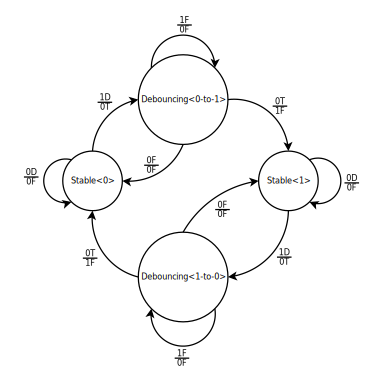
\includegraphics[width=0.9\textwidth, height=\textheight, keepaspectratio=true]{hw04q5c}
\end{center}

\end{raggedright}
\end{document}
